% =====================================================================
%  Theoretical documentation for the SDP solver in
%  github.com/probabilist-jnieminen/gap-maximizing-on-ladders
%
%  Location in repo:  docs/theory/main.tex  (+ references.bib)
%  Compile:           latexmk -pdf main.tex
%                     (or: pdflatex, bibtex, pdflatex, pdflatex)
%  TODO markers:      \todo{...} prints red notes; set \draftnotesfalse
%                     below to hide them all in a clean build.
% =====================================================================
\documentclass[11pt,a4paper]{article}

% ---------- packages ----------
\usepackage[margin=2.5cm]{geometry}
\usepackage{amsmath,amssymb,amsthm,mathtools}
\usepackage{bm}
\usepackage{xcolor}
\usepackage{booktabs}
\usepackage{array}
\usepackage{enumitem}
\usepackage{tikz}
\usepackage{algorithm}
\usepackage{algpseudocode}
\usepackage[colorlinks=true,linkcolor=blue!60!black,
citecolor=green!40!black,urlcolor=blue!60!black]{hyperref}
\usepackage[capitalise,noabbrev]{cleveref}
\setlength{\emergencystretch}{2em}

% ---------- draft notes ----------
\newif\ifdraftnotes
\draftnotestrue   % change to \draftnotesfalse to hide all TODOs
\newcommand{\todo}[1]{\ifdraftnotes{\color{red!70!black}\sffamily[TODO: #1]}\fi}
\newcommand{\figplaceholder}[1]{%
	\fbox{\parbox[c][4cm][c]{0.85\linewidth}{\centering\small\sffamily Placeholder: #1}}}

% ---------- theorem environments ----------
\theoremstyle{plain}
\newtheorem{theorem}{Theorem}[section]
\newtheorem{proposition}[theorem]{Proposition}
\newtheorem{lemma}[theorem]{Lemma}
\newtheorem{corollary}[theorem]{Corollary}
\newtheorem{conjecture}[theorem]{Conjecture}
\theoremstyle{definition}
\newtheorem{definition}[theorem]{Definition}
\newtheorem{example}[theorem]{Example}
\theoremstyle{remark}
\newtheorem{remark}[theorem]{Remark}

% ---------- notation ----------
\newcommand{\R}{\mathbb{R}}
\newcommand{\one}{\mathbf{1}}
\newcommand{\ip}[2]{\left\langle #1,\, #2 \right\rangle}
\newcommand{\simplex}{\Delta}
\newcommand{\Lad}{\mathcal{L}}            % ladder graph L_n
\newcommand{\opt}{\lambda^{\star}}        % optimal value
\newcommand{\code}[1]{\texttt{#1}}
\DeclareMathOperator{\tr}{tr}
\DeclareMathOperator{\Diag}{Diag}
\DeclareMathOperator{\rank}{rank}
\DeclareMathOperator{\mult}{mult}
\DeclareMathOperator{\Aut}{Aut}

% =====================================================================
\title{Gap-optimal conductances on ladder graphs \\[4pt]
\large Theoretical documentation of the SDP solver in \code{gap-maximizing-on-ladders}}
\author{Joona Nieminen}
\date{Draft --- \today}

\begin{document}
	\maketitle
	
	\begin{center}
		\small
		\begin{tabular}{ll}
			\toprule
			Repository & \url{github.com/probabilist-jnieminen/gap-maximizing-on-ladders} \\
			Code version documented & commit \todo{hash} \quad / tag \todo{v0.x} \\
			Document status & skeleton; sections marked TODO are unwritten \\
			\bottomrule
		\end{tabular}
	\end{center}
	
	\begin{abstract}
		\todo{3--5 sentences.} We document the mathematics behind a numerical solver for the problem of maximizing the algebraic connectivity \(\lambda_2\) of an \(n\)-rung ladder graph over nonnegative edge conductances with unit total budget. We state the problem, its semidefinite programming (SDP) formulation and dual, the optimality conditions used as numerical certificates, a symmetry reduction specific to ladders, and the design decisions and validation tests of the implementation.
	\end{abstract}
	
	\tableofcontents
	
	% =====================================================================
	\section{Introduction and scope}\label{sec:intro}
	
	\paragraph{Purpose.} This document records (i) the mathematical results the solver relies on, with proofs or citations, (ii) the design decisions of the implementation and their reasons, and (iii) how the numerical output is validated.
	
	\paragraph{Scope.} Two-rail ladders \(\Lad_n = P_n \,\square\, P_2\) with \(n\ge 1\) rungs. Generalizations are listed in \cref{sec:open}.
	
	\paragraph{Map from sections to code.}
	\begin{center}
		\small
		\begin{tabular}{@{}lll@{}}
			\toprule
			Section & Content & Module(s) \\
			\midrule
			\Cref{sec:prelim} & graph, incidence matrix, Laplacian
			& \code{ladder.py}, \code{laplacian.py} \\
			\Cref{sec:sdp,sec:duality} & SDP, dual, certificates
			& \code{solver.py} \todo{confirm name} \\
			\Cref{sec:symmetry} & symmetry-reduced SDP & \todo{module} \\
			\Cref{sec:numerics} & solver pipeline, post-processing & \todo{module} \\
			\Cref{sec:validation} & tests & \code{tests/} \\
			\bottomrule
		\end{tabular}
	\end{center}
	
	\paragraph{Physical motivation.} See \cref{sec:physics}: by Aldous' spectral gap theorem the problem is equivalent to choosing couplings of a ferromagnetic Heisenberg spin ladder that maximise its spectral gap.
	
	% =====================================================================
	\section{Preliminaries}\label{sec:prelim}
	
	\subsection{Weighted graphs and Laplacians}
	
	Let \(G=(V,E)\) be a finite connected simple graph, \(N=|V|\), \(m=|E|\). Fix an arbitrary orientation of each edge \(e = (i,j)\)
	and let \(b_e = \bm e_i - \bm e_j\in\R^V\), \(\bm e_i\) denoting the \(i\)-th standard basis vector (not to be mistaken for the edge \(e\)). The \emph{incidence matrix} \(B\in\R^{E\times V}\) has rows \(b_e^\top\). Denote \(\mathcal{S}_E := [0,1]^E\), then for an arbitrary enumeration of \(E\), let a \emph{conductance vector} \(w\in\mathcal{S}_E\) assign every edge in \(E\) a conductance between \(0\) and \(1\) based on its index in the enumeration. Define
	\begin{equation}\label{eq:laplacian}
		L(w) \;=\; B^\top \Diag(w)\, B \;=\; \sum_{e\in E} w_e\, L_e,
		\qquad L_e := b_e b_e^\top .
	\end{equation}
	For \(e = (i,j)\), the image of said edge \(e\) under \(w\) will occasionally be denoted with \(w_e := w_{ij}\).
	\begin{lemma}[Basic properties]\label{lem:laplacian}
		For every \(w\in\mathcal{S}_E\):
		\begin{enumerate}[label=(\alph*)]
			\item\label{basic-prop:a} \(L(w)\) coincides with the weighted graph Laplacian \(D(w)-A(w)\) (weighted degree minus weighted
			adjacency) and does not depend on the chosen orientation;
			\item \(x^\top L(w)\,x = \sum_{(i,j)\in E} w_{ij}(x_i-x_j)^2 \ge 0\);
			\item \(L(w)\one = 0\) and \(\tr L(w) = 2\sum_{e\in E}w_e\);
			\item $w\mapsto L(w)$ is linear.
		\end{enumerate}
	\end{lemma}
	\begin{proof}
		\todo{Entrywise computation of $B^\top\Diag(w)B$; (b) from
			$x^\top L_e x=(b_e^\top x)^2$.} See also \cite{BrouwerHaemers2012}.
		\begin{enumerate}[label=(\alph*)]
			\item 
			\item Using \ref{basic-prop:a},
			\item 
			\item Using basic properties of matrices,
			\begin{align*}
				& L(\alpha w_1 + \beta w_2) = B^\top\Diag\left( \alpha w_1 + \beta w_2 \right)B = B^\top\left( \alpha\Diag(w_1) + \beta\Diag(w_2) \right)B \\
				& = \alpha B^\top\Diag(w_1)B + \beta B^\top\Diag(w_2)B = \alpha L(w_1) + \beta L(w_2).
			\end{align*}
		\end{enumerate}
	\end{proof}
	
	Order the eigenvalues $0=\lambda_1\le\lambda_2\le\dots\le\lambda_N$. The
	\emph{algebraic connectivity} is $\lambda_2(L(w))$ \cite{Fiedler1973}.
	
	\begin{lemma}[Connectivity]\label{lem:connectivity}
		$\lambda_2(L(w))>0$ if and only if the graph $(V,\{e: w_e>0\})$ is
		connected.
	\end{lemma}
	\begin{proof}\todo{Kernel of $L(w)$ = functions constant on components,
			by \cref{lem:laplacian}(b).} \cite{Fiedler1973}
	\end{proof}
	
	\subsection{Variational characterisation}
	
	\begin{lemma}[Courant--Fischer for $\lambda_2$]\label{lem:cf}
		\[
		\lambda_2\bigl(L(w)\bigr)
		\;=\; \min_{\substack{x\perp\one\\ \|x\|=1}} x^\top L(w)\, x
		\;=\; \min_{\substack{x\perp\one\\ \|x\|=1}}
		\sum_{\{i,j\}\in E} w_{ij}(x_i-x_j)^2 .
		\]
	\end{lemma}
	\begin{proof}
		Courant--Fischer \cite[Thm.~4.2.6]{HornJohnson2013} with the eigenvector
		$\one$ of $\lambda_1=0$ removed. \todo{write out}
	\end{proof}
	
	\begin{lemma}[Trace bound]\label{lem:tracebound}
		If $\one^\top w=1$ then $\lambda_2(L(w))\le 2/(N-1)$, with equality iff
		$L(w)$ restricted to $\one^\perp$ is a multiple of the identity.
	\end{lemma}
	\begin{proof}
		$\lambda_2$ is at most the mean of $\lambda_2,\dots,\lambda_N$, which is
		$\tr L(w)/(N-1)=2/(N-1)$ by \cref{lem:laplacian}(c).
	\end{proof}
	
	\subsection{Ladder graphs}
	
	\begin{definition}[Ladder]\label{def:ladder}
		For $n\ge1$, $\Lad_n$ has vertices $(i,s)$, $i\in\{1,\dots,n\}$,
		$s\in\{1,2\}$, and edges
		\begin{itemize}
			\item \emph{rails}: $\{(i,s),(i+1,s)\}$ for $1\le i\le n-1$, conductance
			$\ell^{(s)}_i$;
			\item \emph{rungs}: $\{(i,1),(i,2)\}$ for $1\le i\le n$, conductance $r_i$.
		\end{itemize}
		Thus $N=2n$, $m=3n-2$, and $\Lad_n\cong P_n\,\square\,P_2$.
	\end{definition}
	
	\begin{figure}[ht]
		\centering
		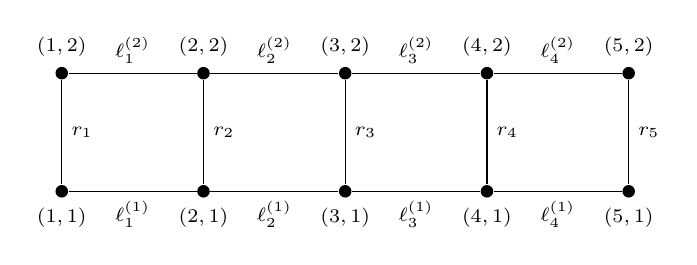
\begin{tikzpicture}[x=1.8cm,y=1.5cm,
			vtx/.style={circle,fill,inner sep=1.6pt}]
			\foreach \i in {1,...,5} {
				\node[vtx,label=below:{\scriptsize$(\i,1)$}] (a\i) at (\i,0) {};
				\node[vtx,label=above:{\scriptsize$(\i,2)$}] (b\i) at (\i,1) {};
				\draw (a\i) -- node[right,font=\scriptsize]{$r_{\i}$} (b\i);
			}
			\foreach \i [evaluate=\i as \j using int(\i+1)] in {1,...,4} {
				\draw (a\i) -- node[below,font=\scriptsize]{$\ell^{(1)}_{\i}$} (a\j);
				\draw (b\i) -- node[above,font=\scriptsize]{$\ell^{(2)}_{\i}$} (b\j);
			}
		\end{tikzpicture}
		\caption{The ladder $\Lad_5$ with its edge labels.}
		\label{fig:ladder}
	\end{figure}
	
	\paragraph{Indexing convention.} \todo{State exactly how vertices $(i,s)$
		and edges map to integer indices and to rail/rung labels in
		\code{ladder.py}, so that formulas here can be checked against the code.}
	
	\begin{example}[Uniform conductances]\label{ex:uniform}
		For $w\equiv 1/m$ the spectrum of $L(w)$ is
		\[
		\Bigl\{\tfrac{1}{3n-2}\bigl(2-2\cos\tfrac{\pi k}{n} + 2s\bigr)
		: 0\le k\le n-1,\ s\in\{0,1\}\Bigr\},
		\]
		since Laplacian spectra add under Cartesian products
		\cite{BrouwerHaemers2012}. Hence
		$\lambda_2^{\mathrm{unif}}=\frac{2-2\cos(\pi/n)}{3n-2}$ for $n\ge2$.
		This is the baseline against which optimised conductances are compared.
	\end{example}
	
	% =====================================================================
	\section{The optimisation problem}\label{sec:problem}
	
	Let $\simplex_E=\{w\in\R^E_{\ge0}:\one^\top w=1\}$. The problem is
	\begin{equation}\label{eq:P}\tag{P}
		\opt(G) \;=\; \max_{w\in\simplex_E}\ \lambda_2\bigl(L(w)\bigr).
	\end{equation}
	
	\begin{proposition}[Concavity]\label{prop:concave}
		$f(w)=\lambda_2(L(w))$ is concave on $\R^E_{\ge0}$, so \eqref{eq:P} is a
		convex optimisation problem.
	\end{proposition}
	\begin{proof}
		By \cref{lem:cf}, $f$ is a pointwise minimum of the linear functions
		$w\mapsto\sum_e w_e(b_e^\top x)^2$. \todo{tidy}
	\end{proof}
	
	\begin{proposition}[Existence and bounds]\label{prop:exist}
		The maximum in \eqref{eq:P} is attained and
		$\lambda_2(L(\one/m))\le\opt(G)\le 2/(N-1)$; in particular $\opt(G)>0$.
	\end{proposition}
	\begin{proof}
		$f$ is continuous and $\simplex_E$ is compact. Lower bound: feasibility of
		$\one/m$ and \cref{lem:connectivity}. Upper bound: \cref{lem:tracebound}.
	\end{proof}
	
	\begin{remark}[Normalisation]
		Fiedler's \emph{absolute algebraic connectivity} \cite{Fiedler1990} uses
		the budget $\one^\top w=m$; by homogeneity it equals $m\,\opt(G)$.
	\end{remark}
	
	\begin{remark}[Nonsmoothness]\label{rem:nonsmooth}
		$f$ is differentiable at $w$ only if $\lambda_2(L(w))$ is simple. At the
		optimum $\lambda_2$ is typically multiple, which is why the problem is
		solved as an SDP rather than by gradient ascent; see also
		\cref{sec:firstorder}.
	\end{remark}
	
	% =====================================================================
	\section{SDP formulation}\label{sec:sdp}
	
	Let $P=I-\frac1N\one\one^\top$ (orthogonal projector onto $\one^\perp$)
	and let $Q\in\R^{N\times(N-1)}$ have orthonormal columns spanning
	$\one^\perp$, so $QQ^\top=P$ and $Q^\top Q=I_{N-1}$.
	
	\begin{lemma}\label{lem:lmi}
		For $w\ge0$ and $t\in\R$ the following are equivalent:
		(i) $\lambda_2(L(w))\ge t$;\;
		(ii) $L(w)-tP\succeq0$;\;
		(iii) $Q^\top L(w)\,Q\succeq t\,I_{N-1}$.
	\end{lemma}
	\begin{proof}
		\todo{$L(w)$ and $P$ commute and share the eigenvector $\one$ (eigenvalue
			$0$ for both); on $\one^\perp$, $P$ acts as the identity.}
	\end{proof}
	
	Consequently \eqref{eq:P} equals each of the SDPs
	\begin{equation}\label{eq:sdpP}\tag{SDP$_P$}
		\begin{aligned}
			\text{maximise}\quad & t\\
			\text{subject to}\quad & L(w)-tP\succeq0,\quad w\ge0,\quad \one^\top w=1,
		\end{aligned}
	\end{equation}
	\begin{equation}\label{eq:sdpQ}\tag{SDP$_Q$}
		\begin{aligned}
			\text{maximise}\quad & t\\
			\text{subject to}\quad & Q^\top L(w)\,Q-tI_{N-1}\succeq0,\quad
			w\ge0,\quad \one^\top w=1,
		\end{aligned}
	\end{equation}
	both of which are linear in $(w,t)$ by \cref{lem:laplacian}(d)
	\cite{VandenbergheBoyd1996,Boyd2006}.
	
	\begin{remark}[Design choice]
		\todo{Which formulation the code uses and why (matrix size $N$ vs.\ $N-1$,
			sparsity of $L(w)$ vs.\ density of $Q$, conditioning, ease of extracting
			the dual). How $Q$ is built, e.g.\ \code{scipy.linalg.null\_space}.}
	\end{remark}
	
	% =====================================================================
	\section{Duality and optimality conditions}\label{sec:duality}
	
	The Lagrange dual of \eqref{eq:sdpP} is
	\begin{equation}\label{eq:D}\tag{D}
		\begin{aligned}
			\text{minimise}\quad & \mu\\
			\text{subject to}\quad & \ip{L_e}{X}\le\mu\quad(e\in E),\qquad
			\ip{P}{X}=1,\qquad X\succeq0 .
		\end{aligned}
	\end{equation}
	\todo{Derive via the Lagrangian $t+\ip{X}{L(w)-tP}+\mu(1-\one^\top w)$.}
	
	\begin{lemma}[Gap identity]\label{lem:gap}
		For $(w,t)$ feasible for \eqref{eq:sdpP} and $(X,\mu)$ feasible for
		\eqref{eq:D},
		\[
		\mu-t \;=\; \ip{L(w)-tP}{X} \;+\; \sum_{e\in E} w_e
		\bigl(\mu-\ip{L_e}{X}\bigr) \;\ge\; 0 .
		\]
	\end{lemma}
	\begin{proof}
		Expand using $\one^\top w=1$ and $\ip{P}{X}=1$; both terms are
		nonnegative. \todo{write out}
	\end{proof}
	
	\begin{theorem}[Strong duality]\label{thm:strong}
		Both \eqref{eq:sdpP} and \eqref{eq:D} attain their optima, and the optimal
		values coincide and equal $\opt(G)$.
	\end{theorem}
	\begin{proof}
		\todo{Slater: $w=\one/m$ with $t<\lambda_2(L(\one/m))$ is strictly
			feasible for the primal; $X=P/(N-1)$ with large $\mu$ for the dual.}
		\cite{VandenbergheBoyd1996,BoydVandenberghe2004}
	\end{proof}
	
	\begin{corollary}[Optimality conditions]\label{cor:kkt}
		Feasible $(w^\star,t^\star)$ and $(X^\star,\mu^\star)$ are optimal iff
		$t^\star=\mu^\star$, iff
		\begin{enumerate}[label=(\roman*)]
			\item $\bigl(L(w^\star)-t^\star P\bigr)X^\star=0$, and
			\item $w^\star_e>0\ \Rightarrow\ \ip{L_e}{X^\star}=\mu^\star$.
		\end{enumerate}
	\end{corollary}
	
	\begin{proposition}[Embedding form of the dual]\label{prop:embedding}
		Without loss of generality $X\one=0$ in \eqref{eq:D}. Writing
		$X=VV^\top$ with rows $v_i\in\R^d$,
		\[
		\frac{1}{\opt(G)} \;=\; \max\Bigl\{\textstyle\sum_{i\in V}\|v_i\|^2 \;:\;
		\sum_{i\in V} v_i=0,\ \ \|v_i-v_j\|\le1\ \ \forall\{i,j\}\in E\Bigr\}.
		\]
	\end{proposition}
	\begin{proof}
		\todo{Replace $X$ by $PXP$ (objective and constraints unchanged since
			$L_eP=L_e$); then $\ip{L_e}{X}=\|v_i-v_j\|^2$ and
			$\ip{P}{X}=\sum_i\|v_i\|^2$; rescale.} This is the ``maximum variance''
		problem of \cite{SunBoydXiaoDiaconis2006,GoeringHelmbergWappler2008}.
	\end{proof}
	
	\begin{remark}[Interpretation]
		By \cref{cor:kkt}(i), every coordinate of an optimal embedding is a
		$\opt$-eigenvector of $L(w^\star)$, so
		$\rank X^\star\le\mult\bigl(\lambda_2(L(w^\star))\bigr)$. By (ii), every
		edge carrying positive conductance has length exactly $1$ in the scaled
		embedding. \todo{Check \cite{GoeringHelmbergWappler2011} for a bound on
			the embedding dimension in terms of tree-width; $\Lad_n$ has tree-width 2.}
	\end{remark}
	
	\begin{remark}[Numerical certificate]\label{rem:certificate}
		Any $w\in\simplex_E$ gives a lower bound $\lambda_2(L(w))\le\opt$ and any
		$X\succeq0$ with $X\one=0$, $\tr X=1$ gives an upper bound
		$\opt\le\max_e\ip{L_e}{X}$. Solver output is repaired to exact
		feasibility (\cref{sec:postprocessing}) to obtain a certified bracket.
	\end{remark}
	
	% =====================================================================
	\section{Symmetry reduction for ladders}\label{sec:symmetry}
	
	\begin{lemma}[Automorphisms]\label{lem:aut}
		For $n\ge3$, $\Aut(\Lad_n)=\langle\sigma,\rho\rangle\cong
		\mathbb Z_2\times\mathbb Z_2$, where $\sigma(i,s)=(i,3-s)$ (rail swap) and
		$\rho(i,s)=(n+1-i,s)$ (reversal). For $n=2$, $\Lad_2\cong C_4$ and the
		group is dihedral of order 8.
	\end{lemma}
	\begin{proof}\todo{Corners are the only vertices of degree 2 \dots}\end{proof}
	
	\begin{proposition}[Symmetric optima exist]\label{prop:symmetrise}
		Let $\Gamma\le\Aut(G)$ and $w^\star$ be optimal for \eqref{eq:P}. Then the
		average $\bar w=\frac1{|\Gamma|}\sum_{\gamma\in\Gamma}\gamma w^\star$ is
		optimal and $\Gamma$-invariant.
	\end{proposition}
	\begin{proof}
		$L(\gamma w)$ is permutation-similar to $L(w)$, so
		$f(\gamma w^\star)=\opt$; $\simplex_E$ is $\Gamma$-invariant; conclude by
		concavity (\cref{prop:concave}). See \cite{GatermannParrilo2004} for
		symmetry reduction of SDPs in general.
	\end{proof}
	
	Hence we may restrict to $\sigma$-invariant conductances
	$\ell_i:=\ell^{(1)}_i=\ell^{(2)}_i$ ($1\le i\le n-1$) and $r_i$
	($1\le i\le n$), with budget $2\,\one^\top\ell+\one^\top r=1$. Let
	$A_\ell$ be the Laplacian of the path $P_n$ with conductances $\ell$, and
	$R=\Diag(r)$.
	
	\begin{proposition}[Sector decomposition]\label{prop:sectors}
		Order vertices as $(1,1),\dots,(n,1),(1,2),\dots,(n,2)$ and let
		$U=\frac1{\sqrt2}\begin{psmallmatrix}I_n&I_n\\I_n&-I_n\end{psmallmatrix}$.
		For $\sigma$-invariant $w$,
		\[
		L(w)=\begin{pmatrix}A_\ell+R & -R\\ -R & A_\ell+R\end{pmatrix},
		\qquad
		U^\top L(w)\,U=\begin{pmatrix}A_\ell & 0\\ 0 & A_\ell+2R\end{pmatrix}.
		\]
	\end{proposition}
	\begin{proof}\todo{Direct block multiplication.}\end{proof}
	
	\begin{corollary}\label{cor:sectors}
		For $\sigma$-invariant $w$,
		\[
		\lambda_2\bigl(L(w)\bigr)
		=\min\bigl\{\lambda_2(A_\ell),\ \lambda_1(A_\ell+2R)\bigr\},
		\]
		with the convention $\lambda_2(A_\ell)=+\infty$ when $n=1$. The first
		term is the \emph{symmetric sector} (rails move together; rungs play no
		role); the second is the \emph{antisymmetric sector}, a discrete
		Schr\"odinger operator on $P_n$ with potential $2r$.
	\end{corollary}
	
	The reduced SDP has two LMIs of sizes $n-1$ and $n$ instead of one of size
	$2n-1$:
	\begin{equation}\label{eq:sdpred}\tag{SDP$_{\mathrm{red}}$}
		\begin{aligned}
			\text{maximise}\quad & t\\
			\text{subject to}\quad & Q_n^\top A_\ell\,Q_n\succeq t\,I_{n-1},\qquad
			A_\ell+2\Diag(r)\succeq t\,I_n,\\
			& \ell\in\R^{n-1}_{\ge0},\quad r\in\R^n_{\ge0},\quad
			2\,\one^\top\ell+\one^\top r=1 .
		\end{aligned}
	\end{equation}
	
	\begin{example}[Closed forms for $n=1,2$]\label{ex:small}
		$n=1$: only the rung, $r_1=1$, so $\opt(\Lad_1)=2$.
		$n=2$: $\lambda_2(A_\ell)=2\ell_1$ and $\lambda_1(A_\ell+2R)=2r$ (with
		$r_1=r_2=r$ by $\rho$-symmetry), under $\ell_1+r=\tfrac12$; hence
		$\ell_1=r=\tfrac14$, i.e.\ uniform conductances, and $\opt(\Lad_2)=\tfrac12$.
	\end{example}
	
	\begin{remark}[Further reduction]
		Imposing $\rho$-invariance ($\ell_i=\ell_{n-i}$, $r_i=r_{n+1-i}$) splits
		each sector further into even and odd parts under reversal.
		\todo{Work out; decide whether worth implementing.}
	\end{remark}
	
	\begin{remark}[Heuristic]
		Budget moved from rails to rungs raises the antisymmetric sector but lowers
		the symmetric one, so at the optimum one expects both sectors to be active,
		i.e.\ $\mult(\lambda_2)\ge2$. \todo{Prove or check numerically.}
	\end{remark}
	
	% =====================================================================
	\section{Physical interpretation: Heisenberg spin ladders}\label{sec:physics}
	
	For couplings $J\in\R^E_{\ge0}$ consider the spin-$\tfrac12$ ferromagnetic
	Heisenberg Hamiltonian on $(\mathbb C^2)^{\otimes V}$,
	\[
	H_J=\sum_{\{i,j\}\in E}J_{ij}\Bigl(\tfrac14-\bm S_i\cdot\bm S_j\Bigr)
	=\tfrac12\sum_{\{i,j\}\in E}J_{ij}\,(1-T_{ij}),
	\]
	where $T_{ij}$ swaps the tensor factors $i$ and $j$.
	
	\begin{theorem}[Aldous' spectral gap conjecture \cite{CaputoLiggettRichthammer2010}]
		The spectral gap of the interchange process with rates $J$ equals that of
		the single random walk, $\lambda_2(L(J))$. Consequently the spectral gap
		of $H_J$ is $\tfrac12\lambda_2(L(J))$ in the normalisation above.
	\end{theorem}
	
	\todo{Align normalisation with the thesis preprint; explain the
		representation-theoretic step (the gap is attained in the standard
		representation, which occurs in $(\mathbb C^2)^{\otimes N}$).} Thus
	\eqref{eq:P} with $G=\Lad_n$ is exactly the problem of gap-optimal
	couplings for a Heisenberg spin ladder under a total-coupling budget.
	
	% =====================================================================
	\section{Numerical method}\label{sec:numerics}
	
	\subsection{Modelling}
	The SDP is written in CVXPY \cite{DiamondBoyd2016}, with $L(w)$ assembled
	as $B^\top\Diag(w)B$ from the NetworkX \cite{HagbergSchultSwart2008}
	incidence matrix. \todo{Short code excerpt or pseudo-code of
		\code{solve\_ladder(n)}; which variables and constraints; how the dual
		$X$ is read from the LMI constraint, including CVXPY's sign and scaling
		conventions.}
	
	\subsection{Solvers and tolerances}
	\begin{center}
		\small
		\begin{tabular}{@{}llp{7cm}@{}}
			\toprule
			Solver & Method & Notes \\
			\midrule
			SCS \cite{ODonoghueChuParikhBoyd2016} & first-order (ADMM)
			& scales to larger $n$; lower accuracy \\
			Clarabel \cite{GoulartChen2024} & interior point
			& open source; higher accuracy \\
			MOSEK & interior point & commercial, free academic licence \\
			\bottomrule
		\end{tabular}
	\end{center}
	\todo{Which solver is the default and why; tolerance values used.}
	
	\begin{center}
		\small
		\begin{tabular}{@{}lll@{}}
			\toprule
			Symbol & Meaning & Value \\
			\midrule
			$\varepsilon_{\mathrm{feas}}$ & feasibility tolerance & \todo{} \\
			$\varepsilon_{\mathrm{supp}}$ & threshold for $w_e>0$ (support) & \todo{} \\
			$\varepsilon_{\mathrm{mult}}$ & eigenvalue clustering for $\mult(\lambda_2)$ & \todo{} \\
			$\varepsilon_{\mathrm{gap}}$ & accepted certified gap $\hat\mu-\hat\lambda$ & \todo{} \\
			\bottomrule
		\end{tabular}
	\end{center}
	
	\subsection{Post-processing and certificates}\label{sec:postprocessing}
	\begin{enumerate}
		\item \emph{Primal repair:} $w\leftarrow\max(w,0)$,
		$w\leftarrow w/\one^\top w$, so $w\in\simplex_E$ exactly.
		\item \emph{Lower bound:} $\hat\lambda=\lambda_2(L(w))$ computed with
		\code{numpy.linalg.eigvalsh}, a dense symmetric eigensolver.
		\item \emph{Dual repair:} clip negative eigenvalues of $X$, replace
		$X\leftarrow PXP/\tr(PXP)$; upper bound
		$\hat\mu=\max_e\ip{L_e}{X}$ (\cref{rem:certificate}).
		\item \emph{Diagnostics:} certified gap $\hat\mu-\hat\lambda$; support
		$\{e:w_e>\varepsilon_{\mathrm{supp}}\}$; $\mult(\lambda_2)$;
		residuals of \cref{cor:kkt}(i)--(ii); optimal embedding from
		the eigendecomposition of $X$.
	\end{enumerate}
	
	\begin{algorithm}[ht]
		\caption{Solve and certify \eqref{eq:P} for $\Lad_n$}\label{alg:solve}
		\begin{algorithmic}[1]
			\Require $n\ge1$; solver $\mathcal S$; tolerances
			\State build $\Lad_n$, $B$, $Q$ \Comment{\code{ladder.py}, \code{laplacian.py}}
			\State solve \eqref{eq:sdpQ} or \eqref{eq:sdpred} with $\mathcal S$;
			read $w$, $t$ and dual $X$
			\State repair $w$ and $X$; compute $\hat\lambda$ and $\hat\mu$
			\If{$\hat\mu-\hat\lambda>\varepsilon_{\mathrm{gap}}$}
			\State flag result as uncertified \Comment{\todo{policy}}
			\EndIf
			\State compute support, $\mult(\lambda_2)$, KKT residuals, embedding
			\State \Return $w$, $[\hat\lambda,\hat\mu]$, diagnostics
		\end{algorithmic}
	\end{algorithm}
	
	\subsection{First-order alternative (optional)}\label{sec:firstorder}
	If $x$ is a unit eigenvector of $L(w)$ for $\lambda_2$ with $x\perp\one$,
	then $g_e=(b_e^\top x)^2$ is a supergradient of $f$ at $w$: indeed
	$f(w')\le x^\top L(w')x=g^\top w'=f(w)+g^\top(w'-w)$. Projected
	supergradient ascent on $\simplex_E$ (projection as in
	\cite{DuchiShalevShwartzSingerChandra2008}) gives a simple solver whose
	iterates can be animated by the visualiser. \todo{Step sizes,
		convergence guarantee, comparison with CVXPY.}
	
	% =====================================================================
	\section{Validation}\label{sec:validation}
	
	\begin{center}
		\small
		\begin{tabular}{@{}p{5.2cm}p{5.6cm}l@{}}
			\toprule
			Test & Checks & File \\
			\midrule
			$L(w)=B^\top\Diag(w)B$ vs.\ NetworkX Laplacian & \cref{lem:laplacian}
			& \todo{} \\
			Uniform spectrum & \cref{ex:uniform} & \todo{} \\
			$n=1$: $\opt=2$; $n=2$: $\opt=\tfrac12$, uniform $w$ & \cref{ex:small}
			& \todo{} \\
			$\lambda^{\mathrm{unif}}_2\le\hat\lambda\le\opt\le\hat\mu\le 2/(2n-1)$
			& \cref{prop:exist,rem:certificate} & \todo{} \\
			certified gap below $\varepsilon_{\mathrm{gap}}$ & \cref{lem:gap,thm:strong}
			& \todo{} \\
			symmetrised solution is optimal & \cref{prop:symmetrise} & \todo{} \\
			full and reduced SDP agree & \cref{cor:sectors} & \todo{} \\
			SCS and Clarabel agree & solver cross-check & \todo{} \\
			\bottomrule
		\end{tabular}
	\end{center}
	
	% =====================================================================
	\section{Numerical observations}\label{sec:observations}
	
	\todo{Fill after Phase 2. Decide what may appear publicly before the
		thesis results are cleared.}
	
	\begin{figure}[ht]
		\centering
		\figplaceholder{optimal rail and rung conductance profiles along the ladder, several $n$}
		\caption{\todo{caption}}\label{fig:profiles}
	\end{figure}
	
	\begin{figure}[ht]
		\centering
		\figplaceholder{$\opt(\Lad_n)$ against $n$ (log--log), with $\lambda_2^{\mathrm{unif}}$ for comparison}
		\caption{\todo{caption}}\label{fig:lambda-vs-n}
	\end{figure}
	
	\begin{conjecture}[Monotonicity]\label{conj:monotone}
		\todo{State precisely.}
	\end{conjecture}
	
	% =====================================================================
	\section{Open questions and extensions}\label{sec:open}
	\begin{itemize}
		\item Asymptotics of $\opt(\Lad_n)$ as $n\to\infty$ and of the optimal
		profiles. \todo{}
		\item Ladders with $k$ rails, $P_n\,\square\,P_k$; circular ladders
		$C_n\,\square\,P_2$.
		\item Other budgets, e.g.\ $\sum_e d_e^2w_e\le1$ as in
		\cite{SunBoydXiaoDiaconis2006}.
		\item Quantum side: \todo{links to the preprint and the QC project}.
	\end{itemize}
	
	% =====================================================================
	\appendix
	
	\section{Notation and code}\label{app:notation}
	\begin{center}
		\small
		\begin{tabular}{@{}lll@{}}
			\toprule
			Symbol & Meaning & Code \\
			\midrule
			$n$ & number of rungs & \code{n} in \code{solve\_ladder(n)} \\
			$\Lad_n$ & ladder graph & \todo{function in \code{ladder.py}} \\
			$B$ & incidence matrix ($m\times N$) & \todo{} \\
			$L(w)$ & weighted Laplacian & \todo{function in \code{laplacian.py}} \\
			$w$; $\ell$, $r$ & conductances; rail and rung parts & \todo{} \\
			$Q$, $P$ & basis of / projector onto $\one^\perp$ & \todo{} \\
			$X$ & dual matrix / Gram matrix of embedding & \todo{} \\
			$\hat\lambda$, $\hat\mu$ & certified lower and upper bounds & \todo{} \\
			\bottomrule
		\end{tabular}
	\end{center}
	
	\section{Design decision log}\label{app:decisions}
	\begin{center}
		\small
		\begin{tabular}{@{}p{3.6cm}p{3.6cm}p{7.2cm}@{}}
			\toprule
			Decision & Alternatives & Reason \\
			\midrule
			NetworkX for graph and incidence matrix; own rail/rung labelling
			& custom graph class
			& established library keeps code short and readable; NetworkX has no
			notion of rails and rungs, hence the small custom layer \\
			$L(w)=B^\top\Diag(w)B$
			& assemble $D-A$ entrywise
			& affine in $w$, so usable directly in CVXPY; matches \cref{lem:laplacian} \\
			CVXPY as modelling layer
			& call a solver API directly
			& near-mathematical syntax; solver can be swapped with one argument \\
			\eqref{eq:sdpP} vs.\ \eqref{eq:sdpQ}
			& \todo{} & \todo{} \\
			default solver & \todo{} & \todo{} \\
			flat package layout (no \code{src/})
			& \code{src/} layout & matches the repository as created \todo{expand} \\
			\bottomrule
		\end{tabular}
	\end{center}
	
	% =====================================================================
	\bibliographystyle{amsplain}
	\bibliography{references}
	
\end{document}